% Wedderburn decomposition of C[S_4] as block-diagonal matrices. Generated by a short script.
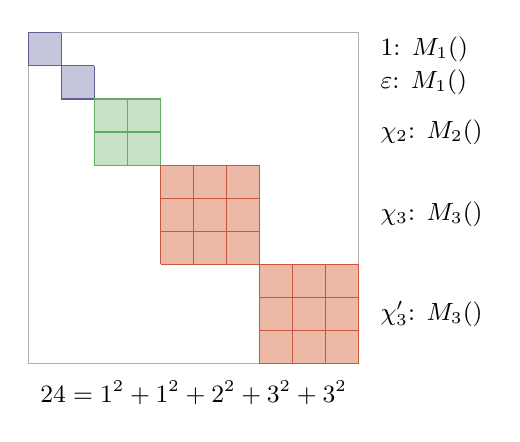
\begin{tikzpicture}[font=\small]
\draw[gray!60] (0,0) rectangle (4.20,-4.20);
\fill[MidnightBlue!25] (0.00,0.00) rectangle (0.42,-0.42);
\draw[MidnightBlue!70] (0.00,0.00) -- (0.42,0.00);
\draw[MidnightBlue!70] (0.00,0.00) -- (0.00,-0.42);
\draw[MidnightBlue!70] (0.00,-0.42) -- (0.42,-0.42);
\draw[MidnightBlue!70] (0.42,0.00) -- (0.42,-0.42);
\node[right] at (4.35,-0.21) {$1$: $M_{1}(\C)$};
\fill[MidnightBlue!25] (0.42,-0.42) rectangle (0.84,-0.84);
\draw[MidnightBlue!70] (0.42,-0.42) -- (0.84,-0.42);
\draw[MidnightBlue!70] (0.42,-0.42) -- (0.42,-0.84);
\draw[MidnightBlue!70] (0.42,-0.84) -- (0.84,-0.84);
\draw[MidnightBlue!70] (0.84,-0.42) -- (0.84,-0.84);
\node[right] at (4.35,-0.63) {$\varepsilon$: $M_{1}(\C)$};
\fill[ForestGreen!25] (0.84,-0.84) rectangle (1.68,-1.68);
\draw[ForestGreen!70] (0.84,-0.84) -- (1.68,-0.84);
\draw[ForestGreen!70] (0.84,-0.84) -- (0.84,-1.68);
\draw[ForestGreen!70] (0.84,-1.26) -- (1.68,-1.26);
\draw[ForestGreen!70] (1.26,-0.84) -- (1.26,-1.68);
\draw[ForestGreen!70] (0.84,-1.68) -- (1.68,-1.68);
\draw[ForestGreen!70] (1.68,-0.84) -- (1.68,-1.68);
\node[right] at (4.35,-1.26) {$\chi_2$: $M_{2}(\C)$};
\fill[BrickRed!25] (1.68,-1.68) rectangle (2.94,-2.94);
\draw[BrickRed!70] (1.68,-1.68) -- (2.94,-1.68);
\draw[BrickRed!70] (1.68,-1.68) -- (1.68,-2.94);
\draw[BrickRed!70] (1.68,-2.10) -- (2.94,-2.10);
\draw[BrickRed!70] (2.10,-1.68) -- (2.10,-2.94);
\draw[BrickRed!70] (1.68,-2.52) -- (2.94,-2.52);
\draw[BrickRed!70] (2.52,-1.68) -- (2.52,-2.94);
\draw[BrickRed!70] (1.68,-2.94) -- (2.94,-2.94);
\draw[BrickRed!70] (2.94,-1.68) -- (2.94,-2.94);
\node[right] at (4.35,-2.31) {$\chi_3$: $M_{3}(\C)$};
\fill[BrickRed!25] (2.94,-2.94) rectangle (4.20,-4.20);
\draw[BrickRed!70] (2.94,-2.94) -- (4.20,-2.94);
\draw[BrickRed!70] (2.94,-2.94) -- (2.94,-4.20);
\draw[BrickRed!70] (2.94,-3.36) -- (4.20,-3.36);
\draw[BrickRed!70] (3.36,-2.94) -- (3.36,-4.20);
\draw[BrickRed!70] (2.94,-3.78) -- (4.20,-3.78);
\draw[BrickRed!70] (3.78,-2.94) -- (3.78,-4.20);
\draw[BrickRed!70] (2.94,-4.20) -- (4.20,-4.20);
\draw[BrickRed!70] (4.20,-2.94) -- (4.20,-4.20);
\node[right] at (4.35,-3.57) {$\chi_3'$: $M_{3}(\C)$};
\node[below] at (2.10,-4.30) {$24=1^2+1^2+2^2+3^2+3^2$};
\end{tikzpicture}
